\chapter{Estimating Feature Saliency Using 2D Saliency Maps \label{2d_saliency_map}}

A saliency map is a model of visual attention using bottom-up features such as intensity, color and orientation of an image.
%A saliency map 111 is a model of visual selective 
%attention using purely bottom-up features of an image like color, 
%intensity and orientation. Another bottom-up feature of visual 
%input is depth, the distance between eye (or sensor) and objects 
%in the visual field.
%However, traditional saliency maps were designed to provide an indication of visual saliency for 2D images with no clue of particular objects or 3D features in the scene.
However, the traditional map provides an indication of saliency for a points on an image and not the saliency of a particular object or 3D feature.
In order to use 2D saliency maps \cite{itti_model_1998} to estimate visual saliency of 3D features in volume visualization, an inverse distance weighting \cite{shepard_two-dimensional_1968} can be applied to divide a 2D saliency map into several feature saliency maps, one for each feature. Subsequently, the visual saliency of each feature can be estimated with the total intensity of each feature saliency map.

The distance between a pixel of each feature and the pixel in the final image is necessary in computing the inverse distance weighting.
Hence, we perform volume rendering of each feature separately, i.e. other intensity ranges in the transfer function are set to zero except for the feature.
These feature images $ P_{i} (i \in \{1,...,n\})$ are rendered with the same settings (viewpoint, screen size etc.) as the final image.
In addition, a 2D saliency map $ S $ of the final image $ P $ is computed using the model by Itti et al. \cite{itti_model_1998}.

Let $ w_{i} $ be the weight of a pixel $ p $ in the $i$-$th$ feature
\[ w_{i} = \frac{ \frac{1}{d_{i}^{m}} }{ \sum_{j=1}^{n} \frac{1}{d_{j}^{m}} } \]
where $ d_{i} $ is the color distance between the pixel $ p $ in the final image and the corresponding pixel $ p_{i} $ in the $i$-$th$ feature image,
$ n $ is the number of features, and
$ m $ is a user-defined coefficient for controlling the bias of the weighting. Pixels with small distances would have larger weights when $ m $ increases. $ m=1 $ is used and the color distance $ d_{i} $ is computed in the LAB color space in our implementation

Then the corresponding pixel $ s_{i} $ in the $i$-$th$  feature saliency map $ S_{i} $ is
\[ s_{i}=w_{i}s \]
where $ s $ is the pixel in the 2D saliency map $ S $ of the final image.

Therefore, we can obtain $ n $ feature saliency maps by performing the above a pixel-wise operation using the 2D saliency map $ S $ and the final image $ P $ along with each feature images $ P_{i} $ respectively.

Figure~\ref{fig:engine_naive} shows an engine block ($ P $) and its two features ($ P_{1} , P_{2} $).
Figure~\ref{fig:engine_naive_saliencemap} shows the 2D saliency map $ S $ and the two feature saliency maps($ S_{1} , S_{2} $) obtained using the above operation.
The saliency maps in Figure~\ref{fig:engine_naive_saliencemap} are enhanced (multiplied by 8) for better contrast in illustrations. However, the original (i.e. not enhanced) saliency maps are used in the actual computation.

In practice, saliency resulting from a visual feature is not sharply delimited by the boundary of the feature, instead strong feature edges tend to attract attention increasing saliency in a small distribution around the edge.
After distributing the 2D saliency map $ S $ into feature saliency maps $ S_{i} (i \in \{1, ... ,n\})$ using the inverse distance weighting, a small amount of bright pixels around the boundary of the engine block remain in the residual saliency image $ S' $, as shown in Figure~\ref{fig:engine_naive_saliencemap_left}~(a).
Let the residual saliency image be $ S' $.
\[ S'=S- \sum_{j=1}^{n} S_{j} \]

We distribute this residual saliency image $ S' $ to the features according to their influence in the region. The influence of the features are approximated by Gaussians of the feature saliency images, as shown in (b) and (c) of Figure~\ref{fig:engine_naive_saliencemap_left}.
%We distribute these values and add them to the feature saliency maps using another weighting based on the Gaussians of the feature saliency maps $ S_{i}$.
Firstly, we apply a Gaussian filter with kernel size $ k $ to each feature saliency map $ S_{i} $ and get a Gaussian image $ G_{i} $.
In practice, the kernel size $ k $ should be large enough in order to allow the resulting Gaussian images to have non-zero pixels cover most of the bright pixels in the residual saliency image $ S' $.
Let $ g_{i} $ be a pixel in the Gaussian image $ G_{i} $.
Secondly, we distribute the residual saliency image $ S' $ into $ n $ images ($ S'_{1} , ... , S'_{n} $).
%\[ G_{i}=Gaussian(S_{i},k) \]
\[ s'_{i} = \frac{ g_{i} }{ \sum_{j=1}^{n} g_{j} }s' \]
where $ s' $ is a pixel in $ S' $.
Figure~\ref{fig:engine_naive_leftgaussian} displays the residual saliency images ($ S'_{1} $, $ S'_{2} $) of the two features on the engine block. 

Thirdly, we pixel-wisely add the image $ S'_{i} $ to the feature saliency map $ S_{i} $ and obtain the total feature saliency map $ T_{i} $ of the $i$-$th$ feature.
\[ T_{i} =S_{i}+S'_{i}\]

Figure~\ref{fig:engine_naive_saliencemap_features} (a) and (b) display the total feature saliency maps of the red feature and the green feature respectively.

Finally, as shown in Figure~\ref{fig:engine_naive_saliencemap_features} (c), we compute the 2D feature saliency using the sum of intensity values of the total feature saliency maps, i.e. $ T_{i}$ for $ i \in \{1, ... ,n\} $.
Hence, the 2D feature saliency of the $i$-$th$  feature is
\[ FS_{i}=\frac{Intensity(T_{i})}{ \sum_{j=1}^{n} Intensity(T_{j}) } \]

A histogram of the 2D feature saliency of the two features of the engine block is shown in Figure~\ref{fig:engine_naive_saliencemap_features} (c).

\begin{figure}
	\centering
	\begin{minipage}{.33\textwidth}
		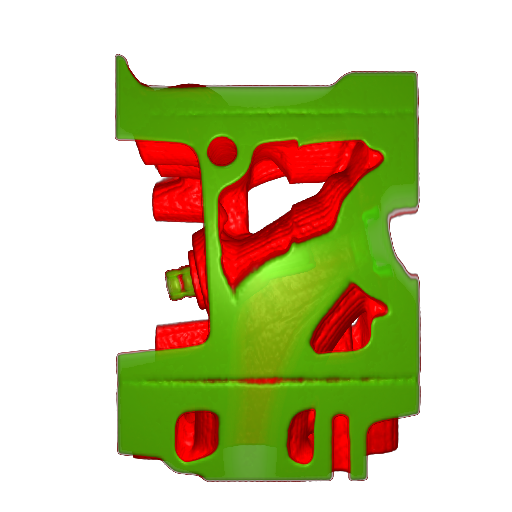
\includegraphics[width=1\linewidth]{images/engine_naive}
		\subcaption{$ P $}
	\end{minipage}~
	\begin{minipage}{.33\textwidth}
		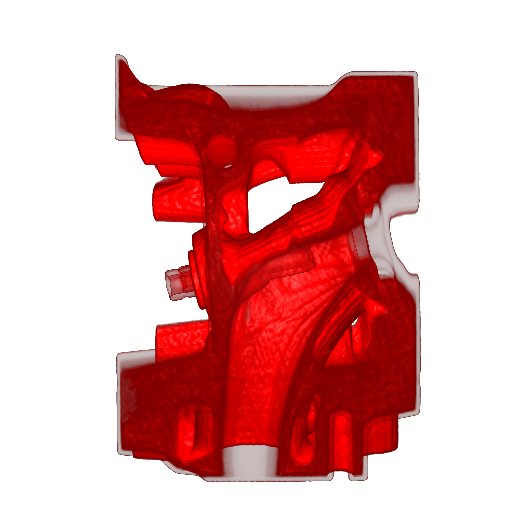
\includegraphics[width=1\linewidth]{images/engine_naive_1}
		\subcaption{$ P_{1} $}
	\end{minipage}~
	\begin{minipage}{.33\textwidth}
		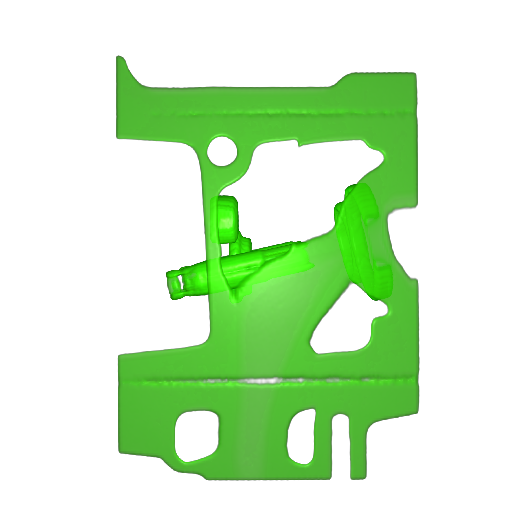
\includegraphics[width=1\linewidth]{images/engine_naive_2}
		\subcaption{$ P_{2} $}
	\end{minipage}
	\caption{(a) An engine block; (b) and (c) isolated volume rendering images of the red feature and the green feature}
	\label{fig:engine_naive}
\end{figure}

\begin{figure}
	\centering
	\begin{minipage}{.33\textwidth}
		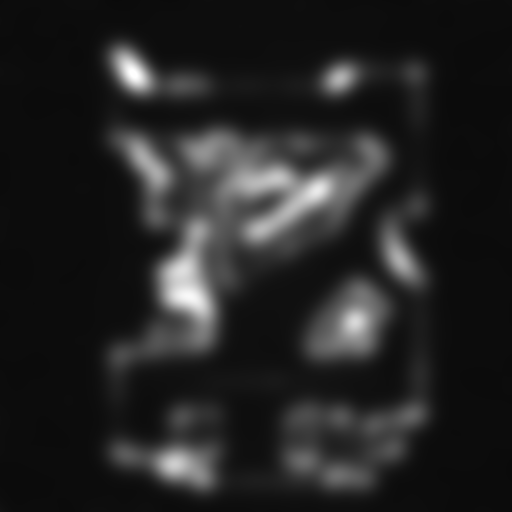
\includegraphics[width=1\linewidth]{images/engine_naive_saliencemap}
		\subcaption{$ S $}
	\end{minipage}~
	\begin{minipage}{.33\textwidth}
		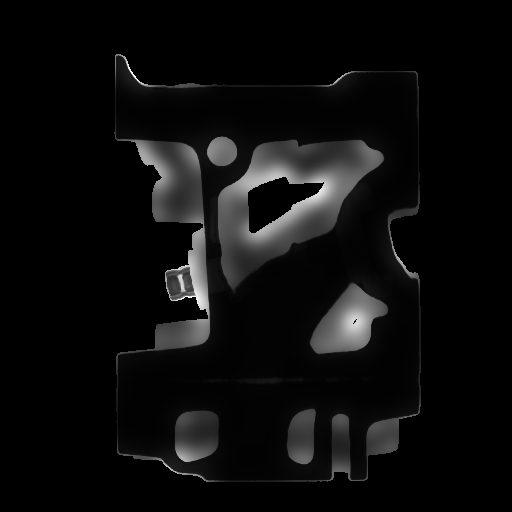
\includegraphics[width=1\linewidth]{images/engine_naive_saliencemap_1_overlap}
		\subcaption{$ S_{1} $}
	\end{minipage}~
	\begin{minipage}{.33\textwidth}
		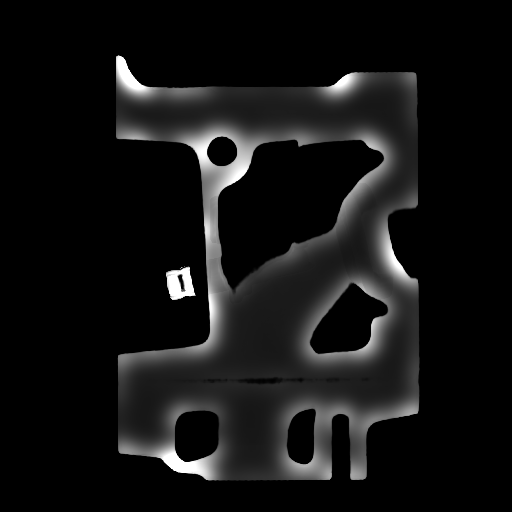
\includegraphics[width=1\linewidth]{images/engine_naive_saliencemap_2_overlap}
		\subcaption{$ S_{2} $}
	\end{minipage}
	\caption[The 2D saliency map and feature saliency maps]{(a) The 2D saliency map; (b) and (c) the feature saliency maps of the two features. The saliency maps are enhanced (multiplied by 8) for better contrast in illustrations.}
	\label{fig:engine_naive_saliencemap}
\end{figure}

\begin{figure}
	\centering
	\begin{minipage}{.33\textwidth}
		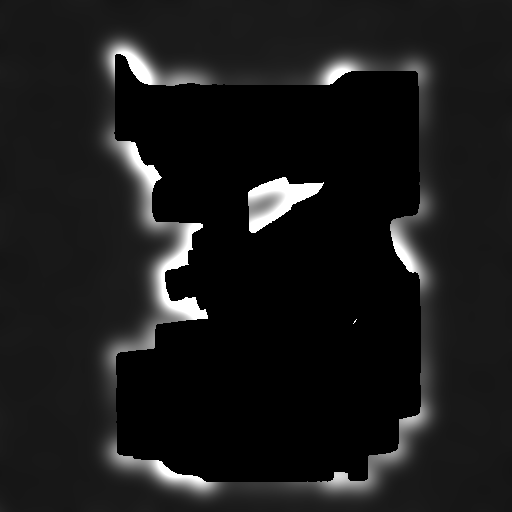
\includegraphics[width=1\linewidth]{images/engine_naive_saliencemap_left}
		\subcaption{$ S' $}
	\end{minipage}~
	\begin{minipage}{.33\textwidth}
		
\includegraphics[width=1\linewidth]{images/engine_naive_gaussian_1}
		\subcaption{$ G_{1} $}
	\end{minipage}~
	\begin{minipage}{.33\textwidth}
		
\includegraphics[width=1\linewidth]{images/engine_naive_gaussian_2}
		\subcaption{$ G_{2} $}
	\end{minipage}
	\caption{(a) The residual saliency image; (b) and (c) the Gaussians of the two feature saliency maps with a kernel size of one eighth of the image width}
	\label{fig:engine_naive_saliencemap_left}
\end{figure}

\begin{figure}
	\centering
	\begin{minipage}{.33\textwidth}
		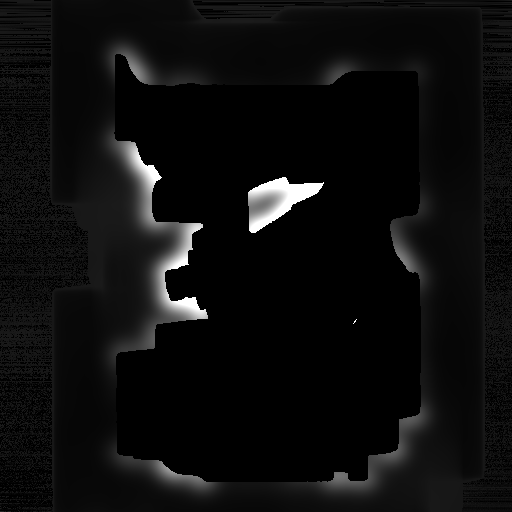
\includegraphics[width=1\linewidth]{images/engine_naive_leftgaussian_1}
		\subcaption{$ S'_{1} $}
	\end{minipage}~
	\begin{minipage}{.33\textwidth}
		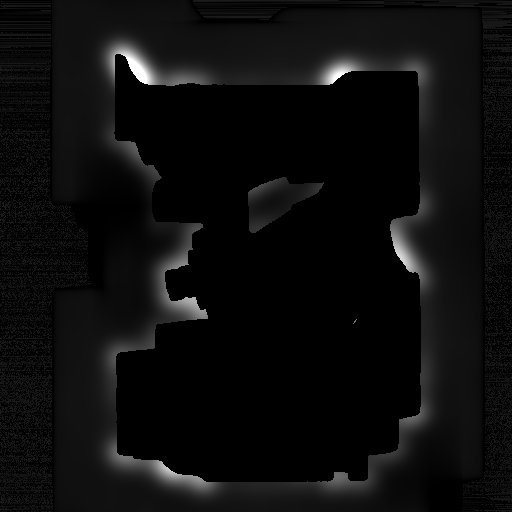
\includegraphics[width=1\linewidth]{images/engine_naive_leftgaussian_2}
		\subcaption{$ S'_{2} $}
	\end{minipage}
	\caption{The residual saliency images of the two features}
	\label{fig:engine_naive_leftgaussian}
\end{figure}

\begin{figure}
	\centering
	\begin{minipage}{.33\textwidth}
		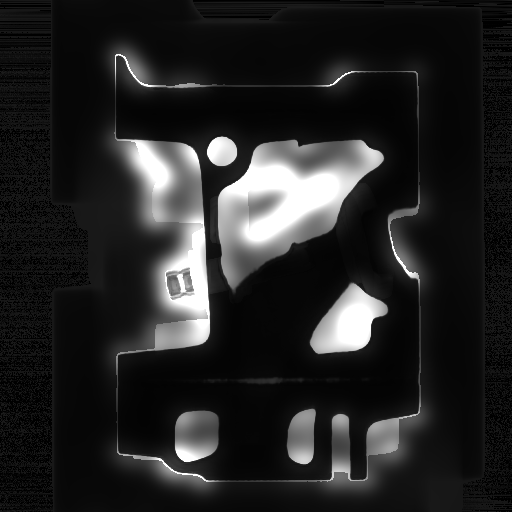
\includegraphics[width=1\linewidth]{images/engine_naive_saliencemap_1}
		\subcaption{$ T_{1} $}
	\end{minipage}~
	\begin{minipage}{.33\textwidth}
		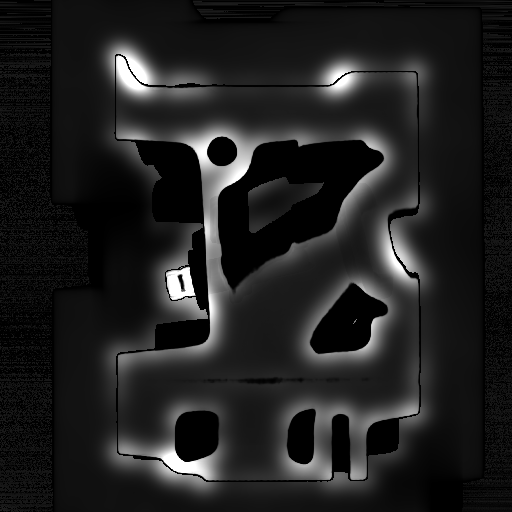
\includegraphics[width=1\linewidth]{images/engine_naive_saliencemap_2}
		\subcaption{$ T_{2} $}
	\end{minipage}~
	\begin{minipage}{.33\textwidth}
		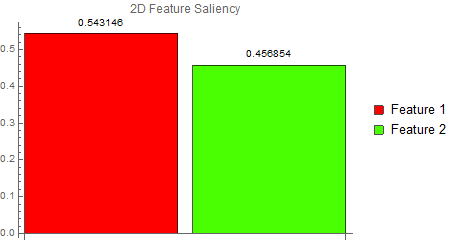
\includegraphics[width=1\linewidth]{images/engine_naive_2DFS}
		\subcaption{2D feature saliency}
	\end{minipage}
	\caption{(a) and (b) The total feature saliency maps of the two features; (c) 2D feature saliency of the two features}
	\label{fig:engine_naive_saliencemap_features}
\end{figure}
